\section{Численный расчёт для одиночного нанодиска}

Расчёты для одиночного нанодиска проводились для гауссова пучка в двух поляризациях: параллельно и перпендикулярно плоскости подложки, при этом X-координата центра диска совпадала с X-координатой центра волновода. Все дальнейшие спектры пропускания волновода представлены нормированными относительно спектра пропускания волновода без диска. Сперва для расчётов была выбрана толщина нанодиска и волновода равная 0.25 мкм, как стандартная высота пластин кремния на изоляторе. К сожалению, при такой конфигурации системы ни для одной из поляризаций не оказалось возможным получить внутри нанодиска распределение локальных полей, отвечающее магнитному резонансу. 

Вышеупомянутое обстоятельство вынудило изменить высоту системы, и таким образом привело к исследованию возможности эффективного возбуждения магнитной моды для наноструктур высотой 0.4 мкм. Так как влияние величины радиуса нанодиска на качественную картину распределения полей внутри него ожидалось более сильным, нежели влияние расстояния между резонатором и волноводом, то в первую очередь была исследована конфигурация системы с наночастицами разных радиусов, вплотную примыкающих к волноводу. Некоторые из спектров пропускания волновода для такого изменения параметров представлены на рисунке \ref{fig:1x_fixed_d}.

\begin{figure}[h]
	\begin{subfigure}[b]{\textwidth}
		\centering
		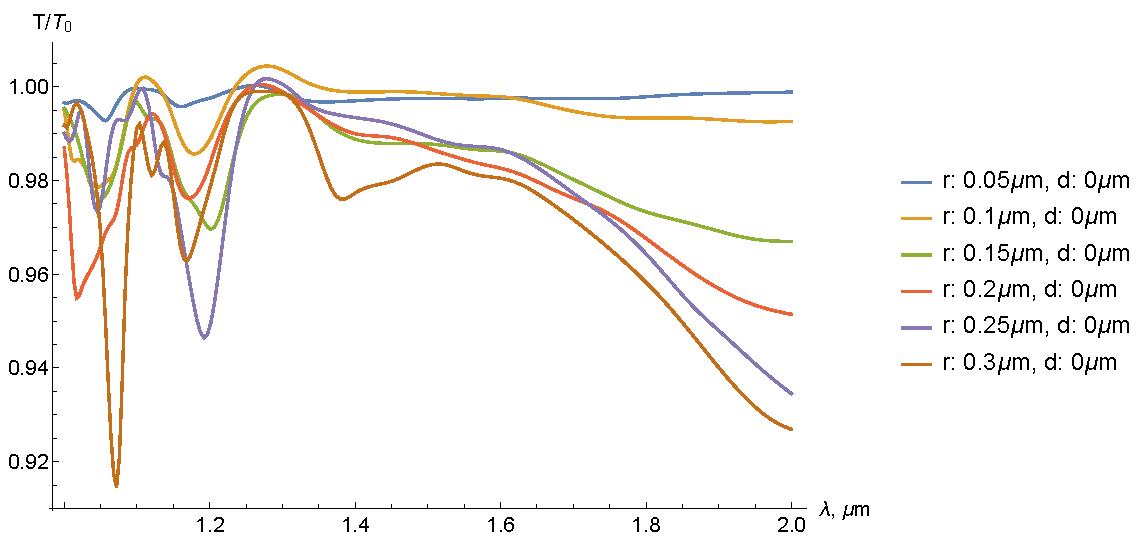
\includegraphics[width=.9\textwidth]{img/total_d0_theta_0}
		\caption{Поляризация, параллельная плоскости подложки}
		\label{fig:1x_fixed_d_theta_0}
	\end{subfigure}

	\begin{subfigure}[b]{\textwidth}
		\centering
		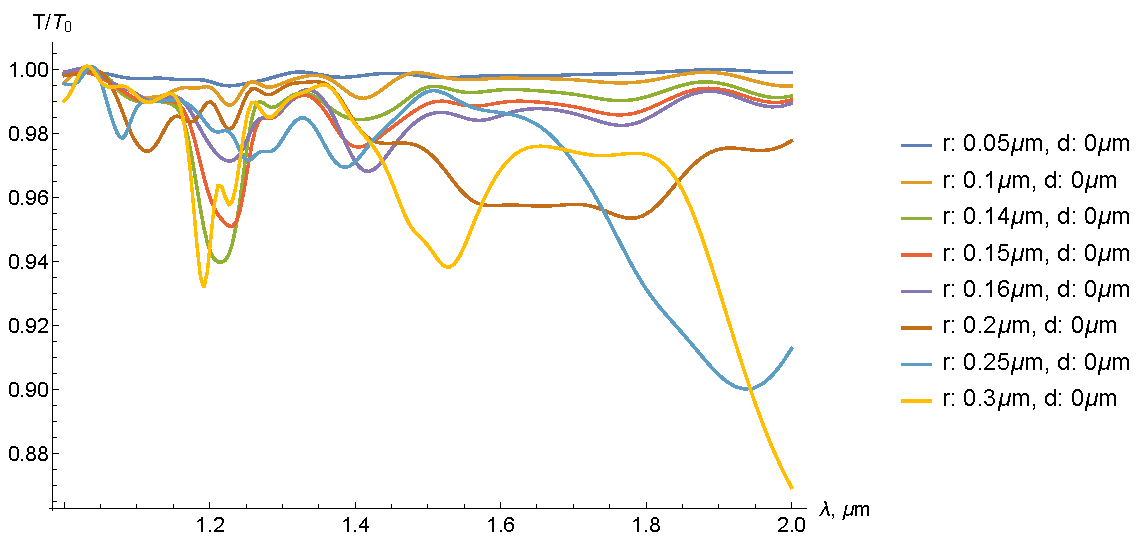
\includegraphics[width=.9\textwidth]{img/total_d0_theta_90}
		\caption{Поляризация, перпендикулярная плоскости подложки}
		\label{fig:1x_fixed_d_theta_90}
	\end{subfigure}
  
  	\caption{Зависимость спектра пропускания от радиуса нанодиска}
  	\label{fig:1x_fixed_d}
\end{figure}

При исследовании распределения полей внутри нанодиска для различных радиусов и поляризаций наиболее эффективное резонансное возбуждение магнитной моды было обнаружено для следующих параметров: поляризация пучка перпендикулярна плоскости подложки, радиус нанодиска равен 0.14 мкм. Графики, иллюстрирующие поведение электрической компоненты поля внутри резонатора для сечения, параллельного плоскости $XZ$ и проходящего через ось симметрии и длины волны равной 1.22 мкм представлены на рисунке \ref{fig:E_reson}.

\begin{figure}[H]
	\begin{subfigure}[b]{.5\textwidth}
		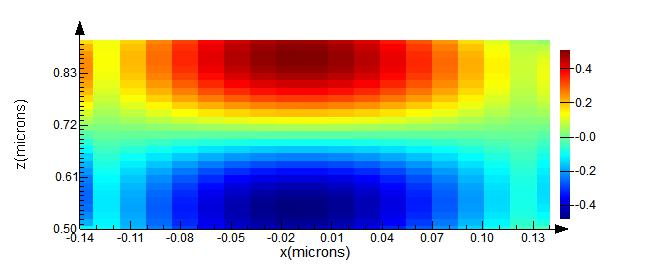
\includegraphics[width=\textwidth]{img/E_x_014}
		\caption{$E_x$}
	\end{subfigure}
	\begin{subfigure}[b]{.5\textwidth}
		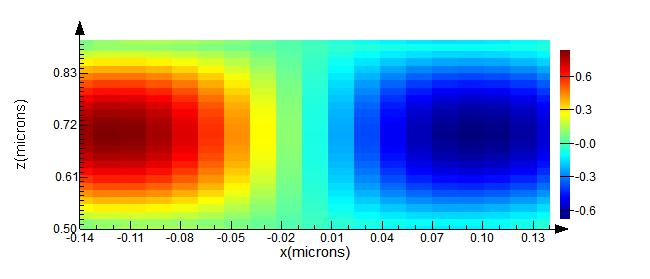
\includegraphics[width=\textwidth]{img/E_z_014}
		\caption{$E_z$}
	\end{subfigure}
	\caption{Распределение электрического поля внутри нанодиска при магнитном резонансе}
	\label{fig:E_reson}
\end{figure}

Далее была проведена оптимизация расстояния между волноводом и нанодиском. Некоторые спектры пропускания волновода при различных расстояниях приведены на рисунке \ref{fig:1x_fixed_r}. При этом в качестве оптимального расстояния была выбрана величина -0.01 мкм.

\begin{figure}[h]
	\centering
	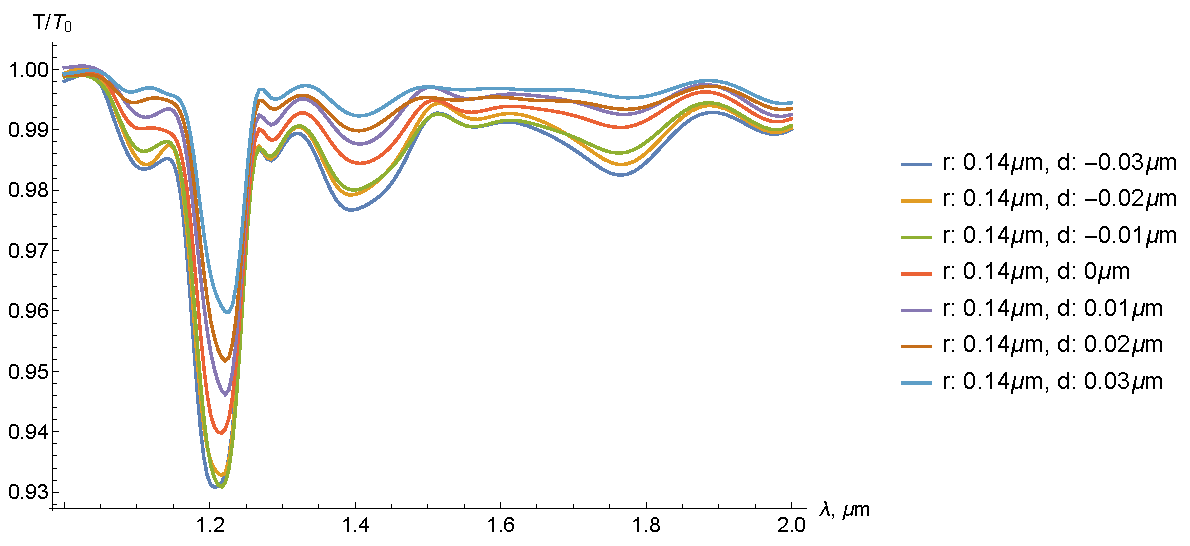
\includegraphics[width=.9\textwidth]{img/r_014_d_var}
	\caption{Зависимость спектра пропускания от расстояния между нанодиском и волноводом}
	\label{fig:1x_fixed_r}
\end{figure}

Таким образом были определены оптимальные параметры системы из волновода и связанного с ним нанодиска для возбуждения магнитной моды в резонаторе. Они приведены в сводной таблице \ref{tbl:effective_params}.

\begin{table}[H]
	\centering
	\begin{tabular}{|c|c|c|}
		\hline
		Плоскость поляризации & Радиус нанодиска & Расстояние между диском и волноводом \\
		\hline
		$XZ$ & 0.14 мкм & -0.01 мкм \\
		\hline
	\end{tabular}
	\caption{Эффективные параметры системы для возбуждения магнитного резонанса}
	\label{tbl:effective_params}
\end{table}
